\documentclass[final,oneside]{book}
\newcommand{\doctitle}{HSA Runtime Programmer's Reference Manual}

% Needed so characters such as underscore are recognized in PDF
% viewers. Otherwise searching for say `hsa_open` produces no
% results
\usepackage[T1]{fontenc}

% Times font definitions
\usepackage{times}

\usepackage[top=2.5cm,bottom=2.5cm,left=2.5cm,right=2.5cm]{geometry}

\usepackage[toc,page]{appendix}
\usepackage[usenames,dvipsnames,svgnames,table]{xcolor}
  \definecolor{lightgray}{gray}{0.94}
\usepackage{makeidx}
\usepackage{pbox}
\usepackage{sidecap}
\usepackage{float}

% overwrite global draft option so the source is shown in draft mode
\usepackage[final]{listings}

% allow tables across page breaks
\usepackage{longtable}

% Use Tikz for simple diagrams
\usepackage{tikz}
\usetikzlibrary{arrows,automata,positioning,chains,shapes.geometric}
\tikzset{
    % define global arrow tip format
    >=angle 45}

% allows width arithmetic, currently used in the LaTeX generated by xml2tex
\usepackage{calc}

% allow usage of underscore w/o resorting to underscore package
% the underscore package imposes more restrictions on where underscores still
% cannot be used (e.g.: labels)
\catcode`_=12 % we need this line, even when it is repeated afterwards
\AtBeginDocument{
   \catcode`_=12
   \begingroup\lccode`~=`_
   \lowercase{\endgroup\let~}\sb
   \mathcode`_="8000
 }

\usepackage{ifthen}
\usepackage{textcomp}

% inline enumerations and itemizes in the paragraph instead of breaking
\usepackage{paralist}

% Customizable headers/footers
\usepackage{fancyhdr}

% add API index. Note that 'imakeidx' works within Latex (unlike 'makeidx', which
% requires running 'makeindex' from command line)
\usepackage{imakeidx}
\makeindex[name=api,title=Index - Core APIs,columns=1,intoc]
\makeindex[name=ext,title=Index - Extension APIs,columns=1,intoc]

% allows customization of description environment (margin, indentation, etc.)
\usepackage{enumitem}

\lstset{% in alphabetical order
        backgroundcolor=\color{lightgray},
        basicstyle=\footnotesize,
        breakatwhitespace=true,
        breaklines=true,
        captionpos=b,      % sets the caption-position to bottom
        columns=fullflexible,
        commentstyle=\color{ForestGreen},
        emphstyle={\textbf},
        frame=single,
        framexbottommargin=3pt, % bottom frame padding
        framextopmargin=3pt, % top frame padding
        inputencoding=utf8,
        keywordstyle=\color{Blue},
        language=C,
        rulecolor=\color{lightgray}, % invisible (we use it because it allows padding)
        showstringspaces=false,
        tabsize=4,
}
% prevent listings package from changing hyphens to minus signs
\makeatletter
\lst@CCPutMacro\lst@ProcessOther {"2D}{\lst@ttfamily{-{}}{-{}}}
\@empty\z@\@empty
\makeatother
% Use Example instead of Listing in captions
\renewcommand{\lstlistingname}{Example}
% List of Listings -> List of Examples
\renewcommand{\lstlistlistingname}{List of \lstlistingname s}
% include automatically-generated Listing commands
\input{api/altlatex/listings}

\input{example/altlatex/lstinputfunlisting}

% formatting of arguments, function names, types, etc.
% remember to add this commands to the safe command list of Latexdiff so
% it includes them in the diff algorithm
\newcommand{\reffun}[1]{\textbf{#1}}
\newcommand{\refarg}[1]{\textit{#1}}
\newcommand{\reffld}[1]{\textit{#1}}
\newcommand{\reftyp}[1]{#1}
\newcommand{\refenu}[1]{\reftyp{#1}}
\newcommand{\refhsl}[1]{\reffun{#1}}

% allows string comparison, which is used to match \hsaref arguments
\usepackage{pdftexcmds}
% Automatically generated file containing all the definitions in the header that
% can be referenced via \hsaref commands
\input{api/altlatex/commands}

% every section in a new page
\usepackage{etoolbox}
\pretocmd{\section}{%
  \ifnum\value{section}=0 \else\clearpage\fi
}{}{}

% define marginparwidth so todonotes renders properly
\setlength{\marginparwidth}{2cm}
\usepackage[obeyDraft,obeyFinal,textsize=scriptsize]{todonotes}

\usepackage[
            % link color is black
            allcolors=black,
            % Do not use colors or frames in links
            % If colors are used, they overwrite those of the DIFF tool so
            % many differences would not be shown
            hidelinks,
            % use links even if the document is draft
            final,
            %sections and subsections linked
            linktoc=all,
           ]{hyperref}

% alternate rowcolors for all long-tables
\let\oldlongtable\longtable
\let\endoldlongtable\endlongtable
\newenvironment{mylongtable}{\rowcolors{0}{lightgray}{lightgray}\longtable} {
\endlongtable}

% Alter some LaTeX defaults for better treatment of figures:
% See p.105 of "TeX Unbound" for suggested values.
% See pp. 199-200 of Lamport's "LaTeX" book for details.
%   General parameters, for ALL pages:
\renewcommand{\topfraction}{0.9}	% max fraction of floats at top
\renewcommand{\bottomfraction}{0.8}	% max fraction of floats at bottom
%   Parameters for TEXT pages (not float pages):
\setcounter{topnumber}{2}
\setcounter{bottomnumber}{2}
\setcounter{totalnumber}{4}     % 2 may work better
\setcounter{dbltopnumber}{2}    % for 2-column pages
\renewcommand{\dbltopfraction}{0.9}	% fit big float above 2-col. text
\renewcommand{\textfraction}{0.07}	% allow minimal text w. figs
%   Parameters for FLOAT pages (not text pages):
\renewcommand{\floatpagefraction}{0.7}	% require fuller float pages
% N.B.: floatpagefraction MUST be less than topfraction !!
\renewcommand{\dblfloatpagefraction}{0.7}	% require fuller float pages

% push footer a little further away
\setlength{\footskip}{35pt}

% Side notes. One command per author
\newcommand{\mariotodo}[1]{\todo[color=CarnationPink]{#1}}

% Increase paragraph separation
\setlength{\parskip}{2mm}

% no indentation
\setlength{\parindent}{0cm}

% number (sub)sections up to level 3
\setcounter{secnumdepth}{3}

\makeindex
\setcounter{tocdepth}{3}
\renewcommand{\footrulewidth}{0.4pt}
\renewcommand{\familydefault}{\sfdefault}

\RequirePackage[normalem]{ulem}
\newenvironment{DIFnomarkup}{}{}


\makeatletter
\newcommand*{\tidyhdr}[2]{
  % if \rightmark is empty or equal to \leftmark, omit
  \ifnum\pdf@strcmp{#1}{#2}=\z@ #1\else \ifnum\pdf@strcmp{}{#2}=\z@ #1\else #1: #2\fi\fi
}
\makeatother

% header and footer layout
\newcommand{\hfstyle}{
% clear all header and footer fields
\fancyhf{}
\rfoot{\scriptsize{\thepage}}
\lfoot{\scriptsize{\doctitle$\:$v1.00$\:$-$\:$\today}}
\lhead{\scriptsize{\nouppercase{\tidyhdr{\leftmark}{\rightmark}}}}
\renewcommand{\headrulewidth}{0pt}
\renewcommand{\footrulewidth}{0pt}
}

% use custom header and footer
\pagestyle{fancy}
\hfstyle{}
\renewcommand{\chaptermark}[1]{\markboth{#1}{}}
\renewcommand{\sectionmark}[1]{\markright{#1}{}}
\usepackage{datatool}
\newcommand{\sortitem}[2]{%
  \DTLnewrow{list}%
  \DTLnewdbentry{list}{company}{#1}%
  \DTLnewdbentry{list}{description}{#2}%
}
\newcommand*{\processed}{}
\newenvironment{sorteddescription}{%
  \DTLifdbexists{list}{\DTLcleardb{list}}{\DTLnewdb{list}}
}{
  \DTLsort{company,description}{list}
  \begin{description}[itemsep=0pt,leftmargin=0pt, labelindent=0cm]
    \DTLforeach*{list}{\comp=company,\desc=description}{
      \expandafter\DTLifinlist\expandafter{\comp}{\processed}
         {\hspace{-1mm}\desc\\}
         {\ifdefempty{\processed}{\let\processed\comp{\item[\comp]$\;$\\\desc\\}}
         {\eappto\processed{,\comp}{\item[\comp]$\;$\\\desc\\}}% append to list
         }
       }
  \end{description}
}

% plain style is identical to fancy style. This avoids different formatting in
% the first page of every chapter, for example.
\fancypagestyle{plain}{\hfstyle{}}

\begin{document}

% redefine DIFadd command to avoid \uwave, which causes troubles when the
% argument includes \hypertarget or \hyperlink
% also, changing default 'add color' to avoid collisions with lstlistings colors
\providecommand{\DIFadd}[1]{{\protect\color{Cerulean}#1}}
\renewcommand{\DIFadd}[1]{{\protect\color{Cerulean}#1}}

% Surrounding the text with \mbox is the only way \sout can wrap \hyperref or
% \hypertarget; otherwise, we get a compilation error.
% However, mbox'ed text does not respect the page margins, resulting in lines
% that disappear through the right hand-side of the page.
\providecommand{\DIFdel}[1]{{\protect\color{red}\sout{\mbox{#1}}}}
\renewcommand{\DIFdel}[1]{{\protect\color{red}\sout{\mbox{#1}}}}

\pagenumbering{roman}
\addcontentsline{toc}{chapter}{Cover} % add cover to TOC

\begin{titlepage}

\includegraphics[width=.4\textwidth]{fig/foundation.png}
\vspace*{7cm}
\begin{center}
{\Large \doctitle\\[1ex]\large v1.00}\\ % remember to change footer version too!
\vspace*{1cm}
\vspace*{0.5cm}
{\small \today}
\end{center}
\end{titlepage}
\thispagestyle{empty} {\textcopyright 2013-2014 HSA Foundation. All rights
  reserved.}


The contents of this document are provided in connection with the HSA Foundation
specifications. This specification is protected by copyright laws and contains
material proprietary to the HSA Foundation. It or any components may not be
reproduced, republished, distributed, transmitted, displayed, broadcast or
otherwise exploited in any manner without the express prior written permission
of HSA Foundation. You may use this specification for implementing the
functionality therein, without altering or removing any trademark, copyright or
other notice from the specification, but the receipt or possession of this
specification does not convey any rights to reproduce, disclose, or distribute
its contents, or to manufacture, use, or sell anything that it may describe, in
whole or in part.

HSA Foundation grants express permission to any current Founder, Promoter,
Supporter Contributor, Academic or Associate member of HSA Foundation to copy
and redistribute UNMODIFIED versions of this specification in any fashion,
provided that NO CHARGE is made for the specification and the latest available
update of the specification for any version of the API is used whenever
possible. Such distributed specification may be re-formatted AS LONG AS the
contents of the specification are not changed in any way. The specification may
be incorporated into a product that is sold as long as such product includes
significant independent work developed by the seller. A link to the current
version of this specification on the HSA Foundation web-site should be included
whenever possible with specification distributions.

HSA Foundation makes no, and expressly disclaims any, representations or
warranties, express or implied, regarding this specification, including, without
limitation, any implied warranties of merchantability or fitness for a
particular purpose or non-infringement of any intellectual property. HSA
Foundation makes no, and expressly disclaims any, warranties, express or
implied, regarding the correctness, accuracy, completeness, timeliness, and
reliability of the specification. Under no circumstances will the HSA
Foundation, or any of its Founders, Promoters, Supporters, Academic,
Contributors, and Associates members or their respective partners, officers,
directors, employees, agents or representatives be liable for any damages,
whether direct, indirect, special or consequential damages for lost revenues,
lost profits, or otherwise, arising from or in connection with these materials.

\clearpage
{\Huge \textbf{Acknowledgments}}\\[3mm]
This specification is the result of the contributions of many people. Here
is a partial list of the contributors, including the company that they
represented at the time of their contribution:
\begin{sorteddescription}
\sortitem{AMD}{M\'{e}ndez-Lojo, Mario (spec editor)}
\sortitem{AMD}{Tye, Tony}
\sortitem{AMD}{Zhuravlyov, Konstantin}
\sortitem{AMD}{Sander, Ben}
\sortitem{AMD}{Tipparaju, Vinod}
\sortitem{AMD}{Thangirala, Hari}
\sortitem{AMD}{Blinzer, Paul}
\sortitem{Qualcomm}{Howes, Lee}
\sortitem{Qualcomm}{Gaster, Ben}
\sortitem{Qualcomm}{Bourd, Alex}
\sortitem{Qualcomm}{Bellows, Greg}
\sortitem{Qualcomm}{Bin, Lihan}
\sortitem{Qualcomm}{Rychlik, Bob}
\sortitem{Qualcomm}{Simpson, Robert J.}
\sortitem{ARM}{Kovacevic, Djordje}
\sortitem{ARM}{Parker, Jason}
\sortitem{ARM}{Persson, H\r{a}kan}
\sortitem{Imagination}{Aldis, James}
\sortitem{Imagination}{Meredith, Jason}
\sortitem{Imagination}{Howson, John}
\sortitem{Imagination}{Glew, Andy}
\sortitem{Imagination}{McCarthy, James}
\sortitem{Imagination}{Rankilor, Mark}
\sortitem{Mediatek}{Bagley, Richard}
\sortitem{Mediatek}{Ju, Roy}
\sortitem{Mediatek}{Lo, Trent}
\sortitem{Mediatek}{Lin, Jason}
\sortitem{Mediatek}{Hsu, Barz}
\sortitem{Mediatek}{Huang, Emerson}
\sortitem{Mediatek}{Agarwal, Rahul}
\sortitem{Via Alliance Technologies}{Hong, Mike}
\sortitem{Sandia National Laboratories}{Stark, Dylan}
\sortitem{Sandia National Laboratories}{Hammond, Simon D.}
\sortitem{Samsung Electronics}{Kohli, Soma}
\sortitem{Samsung Electronics}{Ryu, Soojung}
\sortitem{Samsung Electronics}{Llamas, Ignacio}
\sortitem{Samsung Electronics}{Shebanow, Michael}
\sortitem{Codeplay}{Potter, Ralph}
\sortitem{Codeplay}{Richards, Andrew (workgroup chair)}
\end{sorteddescription}
\clearpage
\phantomsection
\addcontentsline{toc}{chapter}{Contents} % add to TOC
\tableofcontents

\clearpage
\pagenumbering{arabic}
\setcounter{page}{1}

\chapter{Introduction} \label{index}
\vspace{-7mm}
\section{Overview}\label{overview}
\vspace{-3mm}
Recent heterogeneous system designs have integrated CPU, GPU, and other
accelerator devices into a single platform with a shared high-bandwidth memory
system.  Specialized accelerators now complement general purpose CPU chips and
are used to provide both power and performance benefits.  These
heterogeneous designs are now widely used in many computing markets including
cellphones, tablets, personal computers, and game consoles. The Heterogeneous
System Architecture (HSA) builds on the close physical integration of
accelerators that is already occurring in the marketplace, and takes the next
step by defining standards for uniting the accelerators architecturally. The HSA
specifications include requirements for virtual memory, memory coherency,
architected dispatch mechanisms, and power-efficient signals. HSA refers to
these accelerators as HSA components.

The HSA system architecture defines a consistent base for building portable
applications that access the power and performance benefits of the dedicated HSA
components. Many of these HSA components, including GPUs and DSPs, are capable and
flexible processors that have been extended with special hardware for
accelerating parallel code. Historically these devices have been difficult to
program due to a need for specialized or proprietary programming languages. HSA
aims to bring the benefits of these HSA components to mainstream programming
languages using similar or identical syntax to that which is provided for
programming multi-core CPUs. For more information on the system architecture,
refer to the HSA Platform System Architecture Specification~\cite{sar}.

In addition to the system architecture, HSA defines a portable, low-level,
compiler intermediate language called HSAIL.  A high-level compiler
generates the HSAIL for the parallel regions of code. A low-level compiler
called the finalizer translates the intermediate HSAIL to target machine
code. The finalizer can be run at compile-time, install-time, or run-time. Each
HSA component provides its own implementation of the finalizer.  For more
information on HSAIL, refer to the HSA Programmer's Reference Manual~\cite{prm}.

The final piece of the puzzle is the HSA runtime API.  The runtime is a thin,
user-mode API that provides the interfaces necessary for the host to launch
compute kernels to the available HSA components. This document describes the
architecture and APIs for the HSA runtime. Key sections of the runtime API
include:
\begin{itemize}[itemsep=0pt,topsep=0pt,partopsep=0pt]
\item Error handling
\item Runtime initialization and shutdown
\item System and HSA agent information
\item Signals and synchronization
\item Architected dispatch
\item Memory management
\end{itemize}

The remainder of this document describes the HSA software architecture and
execution model, and includes functional descriptions for all of the HSA APIs
and associated data structures.

\begin{figure}[t]
  \centering
  \tikzstyle{lang}=[rectangle,draw,fill=black!30,align=center,minimum width=1.25cm,minimum height=.75cm]
  \tikzstyle{hsa}=[rectangle,draw,fill=black!10,align=center,minimum height=.75cm]
  \tikzstyle{comp}=[rectangle,draw,minimum height=.75cm]
  \begin{tikzpicture}[thick,auto, node distance=1.5cm]
    \scriptsize
    \node[lang] (l0) {OpenCL\texttrademark \\ app};
    \node[lang,below of=l0] (r0) {OpenCL\texttrademark \\ runtime};

    \node[lang,right of=l0] (l1) {Java \\ app};
    \node[lang,below of=l1] (r1) {JVM};

    \node[inner sep=0,below right=.75cm of l1] (k) {...};

    \node[lang,above right=.75cm of k] (l2) {OpenMP \\ app};
    \node[lang,below of=l2] (r2) {OpenMP \\ runtime};

    \node[lang,right of=l2] (l3) {DSL \\ app};
    \node[lang,below of=l3] (r3) {DSL \\ runtime};

    \node[hsa,minimum width=3.5cm,below=2cm of k] (h) {HSA runtime};
    \node[hsa,minimum width=3cm,right=1.5cm of h] (hf) {HSA finalizer};
    \tiny
    \node[comp, below=.75cm of h.west,anchor=west] (c1) {HSA component 1};
    \node[below=.5cm of h.south,anchor=south]       (cAny)  {...};
    \node[comp,below=.75cm of h.east,anchor=east]  (cN) {HSA component N};

    \path[->]
       (l0) edge (r0)
       (l1) edge (r1)
       (l2) edge (r2)
       (l3) edge (r3)
       (r0.south) edge (h)
       (r1) edge (h)
       (r2) edge (h)
       (r3.south) edge (h)
       (h) edge[dashed] (hf)
    ;
  \end{tikzpicture}
  \caption{HSA Software Architecture}
  \label{fig:swarch}
\end{figure}

Figure~\ref{fig:swarch} shows how the HSA runtime fits into a typical software
architecture stack. At the top of the stack is a programming model such as
OpenCL\texttrademark, Java, OpenMP, or a domain-specific language (DSL). The
programming model must include some way to indicate a parallel region that can
be accelerated. For example, OpenCL has calls to \texttt{clEnqueueNDRangeKernel}
with associated kernels and grid ranges. Java defines stream and lambda APIs,
which provide support for both multi-core CPUs and HSA components. OpenMP
contains OMP pragmas that mark loops for parallel computing and that control
other aspects of the parallel implementation. Other programming models can also
build on this same infrastructure.

The language compiler is responsible for generating HSAIL code for the parallel
regions of code. The code can be pre-compiled before runtime or compiled at
runtime. A high-level compiler can generate the HSAIL before runtime, in which
case, when the application loads the finalizer, converts the HSAIL to machine
code for the target machine. Another option is to run the finalizer when the
application is built, in which case the resulting binary includes the machine
code for the target architecture. The HSA finalizer is an optional component of
the HSA runtime, which can reduce the footprint of the HSA software on systems
where the finalization is done before runtime.

Each language also includes a "language runtime" that connects the language
implementation to the HSA runtime. When the language compiler generates code for
a parallel region, it will include calls to the HSA runtime to set up and
dispatch the parallel region to the HSA Component. The language runtime is also
responsible for initializing the HSA runtime, selecting target devices, creating
execution queues, managing memory. The language runtime may use other HSA
runtime features as well. A runtime implementation may provide optional
extensions. Applications can query the runtime to determine which extensions are
available. This document describes the extensions for Finalization, Linking, and
Images.

The API for the HSA runtime is standard across all HSA vendors. This means that
languages that use the HSA runtime can execute on different vendors' platforms
that support the API. Each vendor is responsible for supplying their own HSA
runtime implementation that supports all of the HSA components in the vendor's
platform. HSA does not provide a mechanism to combine runtimes from different
vendors. The implementation of the HSA runtime may include kernel-level
components (required for some hardware components) or may only include
user-space components (for example, simulators or CPU implementations).

Figure~\ref{fig:swarch} shows the ``AQL'' (Architected Queuing
Language) path that application runtimes use to send commands directly to
HSA components. For more information on AQL, refer to Section~\ref{sec:aql}.


\section{Programming Model}\label{sec:executionmodel}

This section introduces the main concepts behind the HSA programming model by
outlining how they are exposed in the runtime API. In this introductory example
we show the basic steps that are needed to launch a kernel.

The rest of the sections in this specification provide a more formal and
detailed description of the different components of the HSA API, including many
not discussed here.

\subsection{Initialization and HSA Component Discovery}
The first step any HSA application must perform is to initialize the runtime
before invoking any other calls to the API:
\begin{lstlisting}
hsa_init();
\end{lstlisting}
The next step the application performs is to find a device where it can launch
the kernel. In HSA parlance, a regular device is called an \emph{HSA agent}, and if
the HSA agent can run kernels then it is also an \emph{HSA component}. The glossary at
the end of this document contains more precise definitions of these terms. The
HSA API uses opaque handles of type \hsaref{hsa_agent_t} to represent HSA agents and
components.

The HSA runtime API exposes the set of available HSA agents via
\hsaref{hsa_iterate_agents}. This function receives a callback and a buffer from
the application; the callback is invoked once per HSA agent unless it returns a
special 'break' value or an error. In this case, the callback queries an HSA
agent attribute (\hsaref{HSA_AGENT_INFO_FEATURE}) in order to determine whether
the HSA agent is also an HSA component. If this is the case, the HSA component
is stored in the buffer and the iteration ends:

\begin{lstlisting}
hsa_agent_t component;
hsa_iterate_agents(get_component, &component);
\end{lstlisting}
where the application-provided callback \textit{get_component} is:
\begin{lstlisting}
hsa_status_t get_component(hsa_agent_t agent, void* data) {
    uint32_t features = 0;
    hsa_agent_get_info(agent, HSA_AGENT_INFO_FEATURE, &features);
    if (features & HSA_AGENT_FEATURE_KERNEL_DISPATCH) {
        // Store HSA component in the application-provided buffer and return
        hsa_agent_t* ret = (hsa_agent_t*) data;
        *ret = agent;
        return HSA_STATUS_INFO_BREAK;
    }
    // Keep iterating
    return HSA_STATUS_SUCCESS;
}
\end{lstlisting}

Section~\ref{sec:agentinfo} lists the set of available HSA agent and
system-wide attributes, and describes the functions to query them.

\subsection{Queues and AQL packets}
When an HSA application needs to launch a kernel in an HSA component, it does so
by placing an \textit{AQL packet} in a \textit{queue} owned by the HSA
component. A packet is a memory buffer encoding a single command. There are
different types of packets; the one used for dispatching a kernel is named
\emph{Kernel Dispatch} packet.

The binary structure of the different packet types is defined in the HSA
Architecture Specification~\cite{sar} standard. For example, all the packets
types occupy 64 bytes of storage and share a common header, and the Kernel
Dispatch packets should specify a handle to the executable code at offset
32. The packet structure is known to the application (Kernel Dispatch packets
correspond to the \hsaref{hsa_kernel_dispatch_packet_t} type in the HSA API),
but also to the hardware. This is a key HSA feature that enables applications to
launch a packet in a specific HSA agent by simply placing it in one of its
\textit{queues}.

A queue is a runtime-allocated resource that contains a packet buffer and is
associated with a packet processor. The packet processor tracks which packets in
the buffer have already been processed. When it has been informed by the
application that a new packet has been enqueued, the packet processor is able to
process it because the packet format is standard and the packet contents are
self-contained -- they include all the necessary information to run a
command. The \textit{packet processor} is generally a hardware unit that is
aware of the different packet formats.

After introducing the basic concepts related to packets and queues, we can go
back to our example and create a queue in the HSA component using
\hsaref{hsa_queue_create}. The queue creation can be configured in multiple
ways. In the snippet below the application indicates that the queue should
be able to hold 256 packets.
\begin{lstlisting}
hsa_queue_t *queue;
hsa_queue_create(component, 256, HSA_QUEUE_TYPE_SINGLE, NULL, NULL, &queue);
\end{lstlisting}

The next step is to create a packet and push it into the newly created
queue. Packets are not created using an HSA runtime function. Instead, the
application can directly access the packet buffer of any queue and setup a
kernel dispatch by simply filling all the fields mandated by the Kernel Dispatch
packet format (type \hsaref{hsa_kernel_dispatch_packet_t}). The location of the
packet buffer is available in the \hsaref{hsa_queue_t.base_address} field of any
queue:
\begin{lstlisting}
hsa_kernel_dispatch_packet_t* packet = (hsa_kernel_dispatch_packet_t*) queue->base_address;

// Configure dispatch dimensions: use a total of 256 work-items
packet->grid_size_x = 256;
packet->grid_size_y = 1;
packet->grid_size_z = 1;

// Configuration of the rest of the Kernel Dispatch packet is omitted for simplicity
\end{lstlisting}

In a real-world scenario, the application needs to exercise more caution when
enqueuing a packet -- there could be another thread writing a packet to the same
memory location. The HSA API exposes several functions that allow the
application to determine which buffer index to use to write a packet, and when to
write it. For more information on queues, refer to Section~\ref{sec:queues}. For
more information on AQL packets, refer to Section~\ref{sec:aql}.

\subsection{Signals and Packet launch}
The Kernel Dispatch packet is not launched until the application informs the
packet processor that there is new work available. The notification is divided
in two parts:

\begin{enumerate}
\item The type field in the packet header must be
  atomically set to the appropriate value using a release memory ordering. This
  ensures that the modifications to the rest of the packet listed before are
  globally visible before or at the same time the desired packet type is
  visible. One possible implementation of the atomic storage (in GCC) is:
\begin{lstlisting}
__atomic_store_n((uint8_t*) &dispatch_packet->header, (uint8_t) HSA_PACKET_TYPE_KERNEL_DISPATCH, __ATOMIC_RELEASE);
\end{lstlisting}
\item The buffer index where the packet has been written (in the example, zero)
must be stored in the \textit{doorbell signal} of the queue.
\end{enumerate}

A \emph{signal} is a runtime-allocated, opaque object used for communication
between HSA agents in an HSA system. Signals are similar to shared memory
locations containing an integer. HSA agents can atomically store a new integer
value in a signal, atomically read the current value of the signal, etc. using
HSA runtime functions.  Signals are the preferred communication mechanism in an
HSA system because signal operations usually perform better (in terms of power
or speed) than their shared memory counterparts. For more information on
signals, refer to Section~\ref{sec:signals}.

When the runtime creates a queue, it also automatically creates a ``doorbell''
signal that must be used by the application to inform the packet processor of
the index of the packet ready to be consumed. The doorbell signal is contained
in the \hsaref{hsa_queue_t.doorbell_signal} field of the queue. The value of a
signal can be updated using \hsaref{hsa_signal_store_release}:

\begin{lstlisting}
hsa_signal_store_release(queue->doorbell_signal, 0);
\end{lstlisting}

After the packet processor has been notified, the execution of the kernel may
start asynchronously at any moment. The application could simultaneously write
more packets to launch other kernels in the same queue.

In this introductory example, we omitted some important steps in the dispatch
process. In particular, we did not show how to compile a kernel, indicate which
executable code to run in the Kernel Dispatch packet, nor how to pass arguments
to the kernel. However, some relevant differences with other runtime systems and
programming models are already evident.  Other runtime systems provide software
APIs for setting arguments and launching kernels, while HSA architects these at
the hardware and specification level. An HSA application can use regular memory
operations and a very lightweight set of runtime APIs to launch a kernel or in
general submit a packet.


\chapter{HSA Core Programming Guide} \label{coreapi}

This chapter describes the HSA Core runtime APIs, organized by functional
area. For information on definitions that are not specific to any functionality,
refer to Section~\ref{sec:other}. The API follows the requirements listed in the
HSA Programmer's Reference Manual~\cite{prm} and the HSA Platform System
Architecture Specification~\cite{sar}.

Several operating systems allow functions to be executed when a DLL or a shared
library is loaded (for example, DLL main in Windows and GCC
\emph{constructor/destructor} attributes that allow functions to be executed
prior to main in several operating systems). Whether or not the HSA runtime
functions are allowed to be invoked in such fashion may be
implementation-specific and is outside the scope of this specification.

Any header files distributed by the HSA Foundation for this specification may
contain calling-convention specific prefixes such as __cdecl or __stdcall, which
are outside the scope of the API definition.

Unless otherwise stated, functions can be considered thread-safe.

\section{Initialization and Shut Down}\label{sec:init}
When an application initializes the runtime (\hsaref{hsa_init}) for the first
time in a given process, a runtime instance is created. The instance is
reference counted such that multiple HSA clients within the same
process do not interfere with each other. Invoking the initialization routine
$n$ times within a process does not create $n$ runtime instances, but a unique
runtime object with an associated reference counter of $n$. Shutting down the
runtime (\hsaref{hsa_shut_down}) is equivalent to decreasing its reference
counter. When the reference counter is less than one, the runtime object ceases
to exist, and any reference to it (or to any resources created while it was
active) results in undefined behavior.

\subsection{API}
\input{api/altlatex/group-initshutdown}

\section{Runtime Notifications}
\label{sec:error}

The runtime can report notifications (errors or events) synchronously or
asynchronously. The runtime uses the return value of functions in the HSA API to
pass synchronous notifications to the application. In this case, the
notification is a status code of type \hsaref{hsa_status_t} that indicates
success or error.

The documentation of each function defines what constitutes a successful
execution. When an HSA function does not execute successfully, the returned
status code might help determining the source of the error. While some
conditions can be generalized to a certain degree (e.g. failure in allocating
resources), others have implementation-specific explanations. For
example, certain operations on signals (explained in Section~\ref{sec:signals})
can fail if the runtime implementation validates the signal object passed by
the application. Because the representation of a signal is specific to the
implementation, the reported error would simply indicate that the signal is
invalid.

The \hsaref{hsa_status_t} enumeration captures the result of any API function
that has been executed, except for accessors and mutators. Success is
represented by \hsaref{HSA_STATUS_SUCCESS}, which has a value of zero. Error
statuses are assigned positive integers and their identifiers start with the
\refenu{HSA_STATUS_ERROR} prefix. The application may use
\hsaref{hsa_status_string} to obtain a string describing a status code.

The runtime passes \textit{asynchronous} notifications in a different fashion.
When the runtime detects an asynchronous event, it invokes an
application-defined callback. For example, queues (described in
Section~\ref{sec:queues}) are a common source of asynchronous events because the
tasks queued by an application are asynchronously consumed by the packet
processor. When the runtime detects an error in a queue, it invokes the callback
associated with that queue and passes it a status code (indicating what
happened) and a pointer to the erroneous queue. An application can associate a
callback with a queue at creation time.

The application must use caution when using blocking functions within their
callback implementation -- a callback that does not return can render the
runtime state to be undefined. The application cannot depend on thread local
storage within the callbacks implementation and may safely kill the thread that
registers the callback. The application is responsible for ensuring that
the callback function is thread-safe. The runtime does not implement any default
callbacks.

\subsection{API}
\input{api/altlatex/group-status}

\section{System and HSA Agent Information}
\label{sec:agentinfo}

The HSA runtime API uses opaque handles of type \hsaref{hsa_agent_t} to
represent HSA agents. The application can traverse the list of HSA agents that
are available in the system using \hsaref{hsa_iterate_agents}, and use
\hsaref{hsa_agent_get_info} to query HSA agent-specific attributes. Examples of
HSA agent attributes include: name, type of backing device (CPU, GPU), and
supported queue types.

If an HSA agent supports Kernel Dispatch packets, then it is also an HSA
component (supports the AQL packet format and the HSAIL instruction set). The
application can inspect the \hsaref{HSA_AGENT_INFO_FEATURE} attribute in order
to determine if the HSA agent is an HSA component. HSA components expose a rich
set of attributes related to kernel dispatches such as wavefront size or maximum
number of work-items in the grid.

Implementations of \hsaref{hsa_iterate_agents} are required to at least report:
\begin{itemize}[itemsep=1pt,topsep=3pt,partopsep=0pt]
\item The host (CPU) HSA agent
\item One HSA component
\end{itemize}

The application can use \hsaref{hsa_system_get_info} to query system-wide
attributes. Note that the value of some attributes is not constant. For example,
the current timestamp (\hsaref{HSA_SYSTEM_INFO_TIMESTAMP}) value returned by the
runtime can increase as time progresses. For more information on timestamps,
please refer to~\cite{sar}, Section 2.5.

\subsection{API}
\input{api/altlatex/group-agentinfo}

\section{Signals}\label{sec:signals}

HSA agents can communicate with each other by using coherent shared (global)
memory or by using signals. HSA agents can perform operations on signals similar
to operations performed on shared memory locations. For example, an HSA agent
can atomically store an integer value on them, atomically load their current
value, etc. However, signals can only be manipulated using the HSA runtime API
or HSAIL instructions. The advantage of signals over shared memory is that
signal operations usually perform better in terms of power or speed. For
example, a spin loop involving atomic memory operations that waits for a shared
memory location to satisfy a condition can be replaced with an HSA signal wait
operator such as \hsaref{hsa_signal_wait_acquire}, which is implemented by the
runtime using efficient hardware features.

The runtime API uses opaque signal handlers of type \hsaref{hsa_signal_t} to
represent signals. A signal carries a signed integer value of type
\reftyp{hsa_signal_value_t} that can be accessed or conditionally waited upon
through an API call or HSAIL instruction. The value occupies four or eight bytes
depending on the machine model (small or large, respectively) being used. The
application creates a signal using the function \hsaref{hsa_signal_create}.

Modifying the value of a signal is equivalent to sending the signal. In addition
to the regular update (store) of a signal value, an application can perform
atomic operations such as add, subtract, or compare-and-swap. Each read or write
signal operation specifies which memory order to use. For example, store-release
(\hsaref{hsa_signal_store_release} function) is equivalent to storing a value on
the signal with release memory ordering. The combinations of actions and
memory orders available in the API match the corresponding HSAIL
instructions. For more information on memory orders and the HSA memory model,
please refer to the other HSA specifications~\cite{prm, sar}.

The application may wait on a signal, with a condition specifying the terms of
the wait. The wait can be done either in the HSA component by using an HSAIL
\refhsl{wait} instruction or in the host CPU by using a runtime API
call. Waiting for a signal implies reading the current signal value (which is
returned to the application) using an acquire (\hsaref{hsa_signal_wait_acquire})
or a relaxed (\hsaref{hsa_signal_wait_relaxed}) memory order. The signal value
returned by the wait operation is not guaranteed to satisfy the wait condition
due to multiple reasons:
\begin{itemize}[itemsep=1pt,topsep=3pt,partopsep=0pt]
\item A spurious wakeup interrupts the wait.
\item The wait time exceeded the user-specified timeout.
\item The wait time exceeded the system timeout
  \hsaref{HSA_SYSTEM_INFO_SIGNAL_MAX_WAIT}.
\item The wait has been interrupted because the signal value satisfies the
  specified condition, but the value is modified before the implementation of
  the wait operation has the opportunity to read it.
\end{itemize}


\subsection{API}

% Macro-dependent typedefs are not showing up correctly in the XML generated
% by Doxygen, so we need to hardcode them :-(
\subsubsection{hsa_\-signal_\-value_\-t}
\vspace{-3.5mm}\begin{mylongtable}{@{}p{\textwidth}}
\rule{0pt}{3ex}\hypertarget{group__signals_1ga67ca2818879c9990e1b5f1b14ce7ed27}{}
\#ifdef HSA_LARGE_MODEL\\
\hspace{1.7em}typedef int64_\-t  \textbf{hsa_\-signal_\-value_\-t}\\
\#else \\
\hspace{1.7em}typedef int32_\-t  \textbf{hsa_\-signal_\-value_\-t}\\
\#endif\rule[-2ex]{0pt}{0pt}
\end{mylongtable}
\vspace{-3mm}Signal value. The value occupies 32 bits in small machine mode, and 64 bits in large machine mode.
\\

\input{api/altlatex/group-signals}

\section{Queues} \label{sec:queues}

HSA hardware supports command execution through user mode queues. A user mode
command queue is characterized~\cite{sar} as runtime-allocated, user-level,
accessible virtual memory of a certain size, containing packets (commands)
defined in the Architected Queueing Language (AQL is explained in more detail in
the next section). A queue is associated with a specific HSA agent. An HSA agent may
have several queues attached to it. We will refer to user mode queues as just
queues.

The application submits a packet to the queue of an HSA agent by performing the
following steps:
\begin{enumerate}[itemsep=1pt,topsep=3pt,partopsep=0pt]

\item Create a queue on the HSA agent, using \hsaref{hsa_queue_create}. The queue
  should support the desired packet type. When the queue is created, the runtime
  allocates memory for the \hsaref{hsa_queue_t} data structure that represents
  the visible part of the queue, as well as the AQL packet buffer pointed by the
  \hsaref{hsa_queue_t.base_address} field.

\item Reserve a packet ID by incrementing the write index of the queue, which is
  a 64-bit unsigned integer that contains the number of packets allocated so
  far. The runtime exposes several functions such as
  \hsaref{hsa_queue_add_write_index_acquire} to increment the value of the write
  index.

\item Wait until the queue is not full (has space for the packet) before writing
the packet. If the queue is full, the packet ID obtained in the previous step
will be greater or equal than the sum of the current read index plus the queue
size. The read index of a queue is a 64-bit unsigned integer that contains the
number of packets that have been processed and released by the queue's packet
processor (i.e., the identifier of the next packet to be released). The
application can load the read index using
\hsaref{hsa_queue_load_read_index_acquire} or
\hsaref{hsa_queue_load_read_index_relaxed}.

  If the application observes that the read index matches the write index, the
  queue can be considered empty. This does not mean that the kernels have
  finished execution, just that all packets have been consumed.

\item Populate the packet. This step does not require using any HSA
  API. Instead, the application directly writes the contents of the AQL packet
  located at \hsaref{hsa_queue_t.base_address} + (AQL packet size) * ((packet
  ID) \% \hsaref{hsa_queue_t.size}). Note that \hsaref{hsa_queue_t.base_address}
  and \hsaref{hsa_queue_t.size} are fields in the queue structure, while the
  size of any AQL packet is 64 bytes. The different packet types are discussed
  in the next section.

\item Launch the packet by first setting the type of the packet field on its
  header to the corresponding value, and then storing the packet ID in
  \hsaref{hsa_queue_t.doorbell_signal} using \hsaref{hsa_signal_store_release}
  (or any variant that uses a different memory order). The application is
  required to ensure that the rest of the packet is globally visible before or
  at the same time the type is written.

  The doorbell signal of the queue is used to indicate the packet processor that
  it has work to do. The value which the doorbell signal must be signaled with
  corresponds to the identifier of the packet that is ready to be launched.
  However, the packet might be consumed by the packet processor even before the
  doorbell signal has been signaled. This is because the packet processor might
  be already processing some other packet and observes that there is new work
  available, so it processes the new packets. In any case, HSA agents are
  required to signal the doorbell for every batch of packets they write.

\item (Optional) Wait for the packet to be complete by waiting on its completion
  signal, if any.

\item (Optional) Submit more packets by repeating steps 2-6

\item Destroy the queue using \hsaref{hsa_queue_destroy}.
\end{enumerate}

Queues are semi-opaque objects: there is a visible part, represented by the
\hsaref{hsa_queue_t} structure and the corresponding ring buffer (pointed to by
\hsaref{hsa_queue_t.base_address}), and an invisible part, which contains at
least the read and write indexes. The access rules for the different queue parts
are:
\begin{itemize}[itemsep=1pt,topsep=3pt,partopsep=0pt]
\item The {hsa_queue_t} structure is read-only. If the application overwrites
  its contents, the behavior is undefined.
\item The ring buffer can be directly accessed by the application.
\item The read and write indexes of the queue can only be accessed using
  dedicated runtime APIs.  The available index functions differ on the index of
  interest (read or write), action to be performed (addition, compare and swap,
  etc.), and memory order applied(relaxed, release, etc.).
\end{itemize}


% \begin{figure}[t]
%   \centering
%   \scriptsize
%   \begin{tikzpicture}[auto,on grid,node distance=5cm,state/.style={circle,draw,minimum size=40pt}]
%     \node[state]                 (s0) {Active};
%     \node[state,dashed,align=center,right=of s0]       (s1) {Error\\Pending\\Inactive};
%     \node[state,align=center,right=of s1]       (s2) {Error\\Inactive};
%     \node[state,accepting,double distance=1pt,below=3cm of s1]   (s3) {Destroyed};
%     \path[->]
%     % create edge without defining start node
%     (-3,0) edge node {\hsaref{hsa_queue_create}} (s0)

%     ([yshift=-.4em]s0.east) edge  node[below] {error in packet} ([yshift=-.4em]s1.west)
%     ([yshift=+.4em]s0.east) edge node[above] {error in dispatch} ([yshift=+.4em]s1.west)
%     (s0) edge[bend left=20]  node {\hsaref{hsa_queue_inactivate}} (s2)
%          edge  node[left] {\hsaref{hsa_queue_destroy}} (s3)

%     ([yshift=-.4em]s1.east) edge[dashed]  node[below] {pending kernels complete} ([yshift=-.4em]s2.west)
%     ([yshift=+.4em]s1.east) edge[dashed] node[above] {\hsaref{hsa_queue_inactivate}} ([yshift=+.4em]s2.west)
%     (s1) edge[dashed]  node[anchor=center,fill=white] {\hsaref{hsa_queue_destroy}} (s3)

%     (s2) edge  node[right] {\hsaref{hsa_queue_destroy}} (s3)
%          edge[loop right] node[anchor=east,above,yshift=+1.0em,xshift=+1.5em] {\hsaref{hsa_queue_inactivate}} ()
%     ;
%   \end{tikzpicture}
%   \caption{Queue state diagram.}
%   \label{fig:queuestate}
% \end{figure}

% \subsection{Queue States} \label{queue-errors}

% A user mode queue can be in one of the following states:
% \emph{active}, \emph{error pending inactive}, \emph{error inactive} or
% \emph{destroyed}. A state diagram showing the various states and transitions is
% shown in Figure~\ref{fig:queuestate}.

% \begin{description}[itemsep=1pt,leftmargin=0cm, labelindent=0cm]
% \item[Active] When a queue is successfully created using the
%   \hsaref{hsa_queue_create} API, it enters the active state. Packets can be
%   added to the queue and are consumed by the packet processor. The actual
%   initiation of dispatch may depend on the resources available for the
%   dispatch. Writing packets to the queue, updating the write index or ringing
%   the doorbell have an effect only when the queue is in the active state. The
%   queue is not monitored by a packet processor in any other state.
% \item[Error pending inactive] If an error is encountered during packet
%   processing (for example, the packet format is invalid) or dispatch, the packet
%   processor stops. At this point, there might be in-flight kernels and resources
%   (such as segment allocation) that have been setup for a dispatch but have not
%   yet been freed. So the queue is not entirely inactive, but when the
%   asynchronous activity concludes, it will become inactive. A queue in
%   \emph{error pending inactive} state is not considered destroyed. It still
%   needs to be destroyed so that the runtime can reclaim the memory allocated for
%   this queue. If an application provides a callback at the time the application
%   creates the queue, the callback is invoked after the queue is marked inactive.
% \item[Inactive] If all the asynchronous activity concludes, the queue enters the
%   inactive state. A queue can also enter this state when the application
%   explicitly invokes the \hsaref{hsa_queue_inactivate} API (note that the queue
%   error callback can invoke this API). In an inactive state, the queue structure
%   and its packets may be inspected. Only the packets that are between the read
%   index and the write index in the queue structure are considered to be valid
%   for inspection by the application. The packet processor guarantees that all the
%   packets that have been consumed by the packet processor (see
%   Section~\ref{dispatch-packet}) will be notified.  Inactivating a queue that is
%   already in the inactive state has no effect.
% \item[Destroyed] The queue has been destroyed by the application. The queue
%   structure and the associated resources (ring buffer, indexes, etc.) are no
%   longer valid.
% \end{description}
\subsection{Example: a simple dispatch}
In this example, we extend the dispatch code introduced in
Section~\ref{sec:executionmodel} in order to illustrate how packet IDs are
reserved (invocation of \hsaref{hsa_queue_add_write_index_relaxed}), and how the
application can wait for a packet to be complete (invocation of
\hsaref{hsa_signal_wait_acquire}). The application creates a signal with an
initial value of 1, sets the completion signal of the Kernel Dispatch packet to
be the newly created signal, and after notifying the packet processor it waits
for the signal value to become zero. The decrement is performed by the packet
processor, and indicates that the kernel has finished.

\lstinputfunlisting{simple_dispatch}

\subsection{Example: error callback}
The previous example can be slightly modified to illustrate the usage of queue
callbacks. This time the application creates a queue passing a callback function
named \emph{callback}:
\begin{lstlisting}
hsa_agent_t component;
hsa_iterate_agents(get_component, &component);

hsa_queue_t *queue;
hsa_queue_create(component, 4, HSA_QUEUE_TYPE_SINGLE, callback, NULL, &queue);
\end{lstlisting}

The callback prints the ID of the problematic queue, and the string associated
with the asynchronous event:
\lstinputfunlisting{callback}
Let's now assume that the application makes a mistake and submits an invalid
packet to the queue. For example, the AQL packet type is set to an invalid
value. When the packet processor encounters this packet, it will trigger an
error that results in the runtime invoking the callback associated with the
queue. The message printed to the standard output varies depending on the string
returned by \hsaref{hsa_status_string}. A possible output is:
\begin{lstlisting}
Error at queue 0: Invalid packet format
\end{lstlisting}

\subsection{Example: concurrent packet submissions}
In previous examples the packet submission is very simple: there is a unique CPU
thread submitting a single packet. In this example, we assume a more realistic
scenario:
\begin{itemize}[itemsep=1pt,topsep=3pt,partopsep=0pt]
\item Multiple threads concurrently submit many packets to the same queue.
\item The queue might be full. Threads should avoid overwriting queue slots
  containing packets that have not been not processed yet.
\item The number of packets submitted exceeds the size of the queue, so the
  submitting thread has to take wrap-around in consideration.
\end{itemize}

We start by finding an HSA component that allows applications to create queues
supporting multiple producers:
\lstinputfunlisting{get_multi_component}

, and then creating a queue on it. The queue type is now
\hsaref{HSA_QUEUE_TYPE_MULTI} instead of \hsaref{HSA_QUEUE_TYPE_SINGLE}.
\begin{lstlisting}
hsa_agent_t component;
hsa_iterate_agents(get_component, &component);
hsa_queue_t *queue;
hsa_queue_create(component, 4, HSA_QUEUE_TYPE_MULTI, callback, NULL, &queue);
\end{lstlisting}
Each CPU thread submits 1,000 Kernel Dispatch packets by executing the function
listed below. For simplicity, we omitted the code that creates the CPU threads.

\lstinputfunlisting{enqueue}

\subsection{API}
\input{api/altlatex/group-queue}

\section{Architected Queuing Language Packets}\label{sec:aql} The Architected
Queuing Language (AQL) is a standard binary interface used to describe commands
such as a kernel dispatch. An AQL packet is a user-mode buffer with a specific
format that encodes one command. The HSA API does not provide any functionality
to create, destroy or manipulate AQL packets. Instead, the application uses
regular memory operation to access the contents of packets, and user-level
allocators (malloc, for example) to create a packet. Applications are not
required to explicitly reserve storage space for packets because a
queue already contains a command buffer where AQL packets can be written.

The HSA API defines the format of the different packet types: Kernel Dispatch,
Agent Dispatch, Barrier-AND and Barrier-OR. All formats share a common header
\hsaref{hsa_packet_type_t} that describes their type, barrier bit (force the
packet processor to complete packets in order), and other properties.

\subsection{Kernel Dispatch packet}\label{dispatch-packet}

An application uses a Kernel Dispatch packet
(\hsaref{hsa_kernel_dispatch_packet_t}) to submit a kernel to an HSA
component. The packet contains the following bits of information:
\begin{itemize}[itemsep=1pt,topsep=3pt,partopsep=0pt]
\item A pointer to the kernel executable code is stored in
  \hsaref{hsa_kernel_dispatch_packet_t.kernel_object}.
\item A pointer to the kernel arguments is stored in
  \hsaref{hsa_kernel_dispatch_packet_t.kernarg_address}. The application
  populates this field with the address of a global memory buffer previously
  allocated using \hsaref{hsa_memory_allocate}, which contains the dispatch
  parameters. Memory allocation is explained in Section~\ref{sec:memory}, which
  includes an example on how to reserve space for the kernel arguments.
\item Launch dimensions. The application must specify the number of dimensions
  of the grid (which is also the number of dimensions of the work-group), the
  size of each grid dimension, and the size of each work-group dimension.
\item If the kernel uses group or private memory, the application must specify
  the storage requirements in the
  \hsaref{hsa_kernel_dispatch_packet_t.group_segment_size} and
  \hsaref{hsa_kernel_dispatch_packet_t.private_segment_size} fields,
  respectively.
\end{itemize}

The application must rely on information provided by the finalizer to retrieve
the amount of kernarg, group, and private memory used by a kernel. Each
executable symbol (\hsaref{hsa_executable_symbol_t}) associated with a kernel
exposes the kernarg
(\hsaref{HSA_EXECUTABLE_SYMBOL_INFO_KERNEL_KERNARG_SEGMENT_SIZE}), group
(\hsaref{HSA_EXECUTABLE_SYMBOL_INFO_KERNEL_GROUP_SEGMENT_SIZE}) and private
(\hsaref{HSA_EXECUTABLE_SYMBOL_INFO_KERNEL_PRIVATE_SEGMENT_SIZE}) static storage
requirements.

\subsubsection{Example: populating the Kernel Dispatch packet}
Examples of kernel dispatches in previous sections have omitted the setup of the
Kernel Dispatch packet. The code listed below shows how to configure the launch
of a kernel that receives no arguments (the
\hsaref{hsa_kernel_dispatch_packet_t.kernel_object} field is NULL). The
dispatch uses 256 work-items, all in the same work-group along the X dimension.

\lstinputfunlisting{initialize_packet}

\subsection{Agent Dispatch packet}\label{agent-packet}

Applications use Agent Dispatch packets to launch built-in functions in HSA
agents. In Agent Dispatch packets there is no need to indicate the address of
the function to run, the launch dimensions, or memory requirements. Instead, the
application or kernel simply specifies the type of function to be performed
(\hsaref{hsa_agent_dispatch_packet_t.type} field), the arguments
(\hsaref{hsa_agent_dispatch_packet_t.arg}), and when applicable, the memory
location where to store the return value of the function
(\hsaref{hsa_agent_dispatch_packet_t.return_address}). The HSA API defines the
type \hsaref{hsa_agent_dispatch_packet_t} to represent Agent Dispatch packets.

A host application is allowed to submit Agent Dispatch packets to any
destination HSA agent that supports them. However, a more common scenario is
that the producer will be a kernel executing in an HSA component. The following
steps describe the set of actions required from the application, the kernel, and
the destination HSA agent:
\begin{enumerate}[itemsep=1pt,topsep=3pt,partopsep=0pt]
\item (Application) Locate a destination HSA agent that supports Agent Dispatch
  packets. The application must check whether the feature
  \hsaref{HSA_AGENT_FEATURE_AGENT_DISPATCH} is present in an HSA agent.
\item (Application) Create a so-called "service'' queue on the destination HSA
  agent using \hsaref{hsa_queue_create}.
\item (Application) Launch a kernel in an HSA component. The work-items
  executing the kernel have access to the service queue -- for example, it has
  been passed as an argument in a Kernel Dispatch packet.
\item (Kernel) When a work-item needs to execute a given built-in (service), it
  submits an Agent Dispatch packet to the service queue following the steps
  described in Section~\ref{sec:queues}.
\item (Destination Agent) The HSA agent parses the packet, executes the
  indicated service, stores the result in the memory location pointed to by
  \hsaref{hsa_agent_dispatch_packet_t.return_address}, and decrements the
  completion signal if present.
\item (Kernel) The work-item consumes the function's output and proceeds to the
  next instruction.
\end{enumerate}

\subsubsection{Example: application processes allocation service requests from
  HSA component}
In this example, work-items in a kernel can ask the host application to
allocate memory on their behalf. This is useful because there is no HSAIL
instruction to allocate virtual memory. In this scenario, the destination HSA
agent is the application running on the CPU, and the service is memory
allocation.

The application starts by finding a CPU HSA agent where it can create a queue
that supports Agent Dispatch packets:
\lstinputfunlisting{get_agent_dispatch_agent}

An application creates a service queue on the CPU HSA agent:
\lstinputfunlisting[1]{create_service_queue}

The application now creates a regular queue on an HSA component and launches a
kernel in that queue. A pointer to the service queue is passed as an argument to
the Kernel Dispatch packet by placing it into the buffer stored in the
\hsaref{hsa_kernel_dispatch_packet_t.kernarg_address}
field. Section~\ref{sec:memory:global} describes the HSA runtime elements needed
for allocating memory that can be used to pass kernel arguments.

Every time a work-item needs more virtual memory, it will submit an Agent
Dispatch packet to the service queue. The allocation size is stored in the first
element of \hsaref{hsa_agent_dispatch_packet_t.arg}, and
\hsaref{hsa_agent_dispatch_packet_t.return_address} contains the memory address
where the application will store the starting address of the allocation.
Finally, the \hsaref{hsa_agent_dispatch_packet_t.type} is set to an
application-defined code. Let's assume that the allocation service type is
0x8000.

The following example code shows how a thread running on the host might process
the Agent Dispatch packets submitted from the HSA component. The application
waits for the value of the doorbell signal in the service queue to be
monotonically increased. When that happens, the thread processes the next service
request by invoking malloc.

\lstinputfunlisting{process_agent_dispatch}

In practice, processing of Agent Dispatch packets is usually more
complex because the consumer has to take into account multiple-producer
scenarios.

\subsection{Barrier-AND and Barrier-OR packets}\label{barrier-packet}

The Barrier-AND packet (of type \hsaref{hsa_barrier_and_packet_t}) allows an
application to specify up to five signal dependencies and requires the packet
processor to resolve those dependencies before proceeding. The packet processor
will not launch any further packets in that queue until the Barrier-AND packet
is complete. A Barrier-AND packet is complete when all of the dependent signals
have been observed with the value 0 after the Barrier-AND packet launched. It is
not required that all dependent signals are observed to be 0 at the same time.

The Barrier-OR packet (of type \hsaref{hsa_barrier_or_packet_t}) is very similar
to the Barrier-AND packet, but it becomes complete when the packet processor
observes that any of the dependent signals have a value of 0.

\subsubsection{Example: handling dependencies across kernels running in
  different HSA components}
A combination of completion signals and Barrier-AND packets allows expressing
complex dependencies between packets, queues, and HSA agents that are
automatically handled by the packet processors. For example, if kernel $b$
executing in HSA component $B$ consumes the result of kernel $a$ executing in a
different HSA component $A$, then $b$ \textit{depends} on $a$. In HSA, this
dependency can be enforced across HSA components by creating a signal that will
be simultaneously used as \begin{inparaenum}[1\upshape)] \item the completion
  signal of a Kernel Dispatch packet $packet\_a$ corresponding to $a$ \item the
  dependency signal in a Barrier-AND packet that precedes the Kernel Dispatch
  packet $packet\_b$ corresponding to $b$\end{inparaenum}. The packet processor
enforces the task dependency by not launching $packet\_b$ until $packet\_a$ has
completed. The following example illustrates how to programmatically express the
described dependency using the HSA API.
\lstinputfunlisting{barrier}

\subsection{Packet states}\label{packet-states}

\begin{figure}[b]
  \centering
  \scriptsize
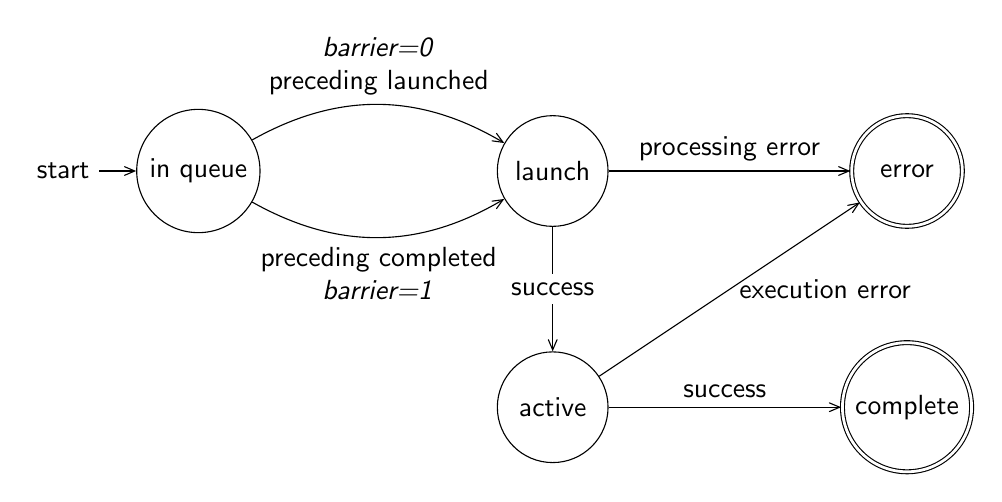
\begin{tikzpicture}
[auto,on grid,node distance=4.5cm,state/.style={circle,draw,minimum size=40pt}]
   \node[state,initial]                 (s0) {in queue};
   \node[state,right=4.5cm of s0]       (s1) {launch};
   \node[state,below=3cm of s1]       (s2) {active};
   \node[state,accepting,double distance=1pt,right=of s1]   (s3) {error};
   \node[state,accepting,double distance=1pt,right=of s2]   (s4) {complete};
   \path[->]
     (s0) edge[bend right]  node[text width=3cm,align=center,below] {preceding completed\\\textit{barrier=1}} (s1)
          edge[bend left] node[text width=3cm,align=center,above]{\textit{barrier=0}\\preceding launched} (s1)
     (s1) edge  node {processing error} (s3)
          edge  node[anchor=center,fill=white,opacity=1] {success} (s2)
     (s2) edge  node{success} (s4)
          edge  node[right]{execution error} (s3)
     ;
\end{tikzpicture}
  \centering
  \caption{Packet State Diagram}
  \label{fig:packetstate}
\end{figure}

After submission, a packet can be in one of the following five states:
\emph{in queue}, \emph{launch}, \emph{error}, \emph{active} or
\emph{complete}. Figure~\ref{fig:packetstate} shows the state transition
diagram.

\begin{description}[itemsep=2pt,leftmargin=0cm, labelindent=0cm] \item[In queue]
  The packet processor has not started to parse the current packet. If the
  barrier bit is set in the header, the transition to the launch state occurs
  only after all the preceding packets have completed their execution. If the
  barrier bit is not set, the transition occurs after the preceding packets have
  finished their launch phase.  In other words, while the packet processor is
  required to launch any consecutive two packets in order, it is not required to
  complete them in order unless the barrier bit of the second packet is set.

\item[Launch] The packet is being parsed, but it has not started execution. This
  phase finalizes by applying an acquire memory fence with the scope indicated
  by the acquire fence scope field in the header. Memory fences are explained
  in~\cite{prm}, Section 6.2.6.

  If an error is detected during launch, the queue transitions to the error
  state and the event callback associated with the queue (if present) is
  invoked. The runtime passes a status code to the callback that indicates the
  source of the problem.  The following status codes can be returned:
  \begin{description}[itemsep=1.5pt,labelindent=.5cm]
  \item[\hsaref{HSA_STATUS_ERROR_INVALID_PACKET_FORMAT}] Malformed AQL
    packet. This can happen if, for example, the packet header type is invalid.
  \item[\hsaref{HSA_STATUS_ERROR_OUT_OF_RESOURCES}] The packet processor is
    unable to allocate the resources required by the launch. This can happen
    if, for example, a Kernel Dispatch packet requests more group memory than
    the size of the group memory declared by the corresponding HSA component.
  \end{description}
\item[Active] The execution of the packet has started.

  If an error is detected during this phase, the queue transitions to the error
  state, a release fence is applied to the packet with the scope indicated by
  the release fence scope field in the header and the event callback associated
  with the queue (if present) is invoked.

  If no error is detected, the transition to the complete state happens when the
  associated task finishes (in the case of Kernel Dispatch and Agent Dispatch
  packets), or when the dependencies are satisfied (in the case of a Barrier-AND
  and Barrier-OR packets).

\item[Complete] A memory release fence is applied with the scope indicated by
  the release fence scope field in the header, and the completion signal (if
  present) decremented.

\item[Error] An error was encountered during the launch or active phases. No
  further packets will be launched on the queue. The queue cannot be recovered,
  but only inactivated or destroyed. If the application passes the queue as an
  argument to any HSA function other than \hsaref{hsa_queue_inactivate} or
  \hsaref{hsa_queue_destroy}, the behavior is undefined.

\end{description}

\subsection{API}
\input{api/altlatex/group-aql}

\section{Memory}\label{sec:memory}

The HSA runtime API provides a compact set of functions for inspecting the
memory \emph{regions} that are accessible from an HSA agent, and (if applicable)
allocating memory on those regions.

A memory region represents a block of virtual memory with certain
characteristics that is accessible by one or more HSA agents. The region object
\hsaref{hsa_region_t} exposes properties about the block of memory such as the
associated memory segment, size, and in some cases allocation characteristics.

The function \hsaref{hsa_agent_iterate_regions} can be used to inspect the set
of regions associated with an HSA agent.  If the application can allocate memory
in a region using the function \hsaref{hsa_memory_allocate}, the flag
\hsaref{HSA_REGION_INFO_RUNTIME_ALLOC_ALLOWED} is set for that region. The HSA
runtime allocator can only be used to allocate memory in the global and readonly
segments. Memory in the private, group and kernarg segments is automatically
allocated when a Kernel Dispatch packet is launched.

When the application no longer needs a buffer that was allocated with the
function \hsaref{hsa_memory_allocate}, it invokes \hsaref{hsa_memory_free} to
release the memory. The application shall not release a runtime-allocated buffer
using standard libraries (such as the function free). Conversely, the runtime
deallocator cannot be used to release memory allocated using standard libraries
(such as the function malloc).

\subsection{Global memory}\label{sec:memory:global}

Regions associated with the global segment are divided into two broad
categories: fine-grained and coarse-grained. The main difference between these
memory types is that fine-grained memory is directly accessible by all the HSA
agents in the system at the same time (under the terms of the HSA memory model),
while coarse-grained memory may be accessible to multiple HSA agents, but never
at the same time: the application is responsible for explicitly assigning
ownership of a buffer to a specific HSA agent. In addition to this, the
application can only use memory allocated from a fine-grained region in order to
pass arguments to a kernel, but not all fine-grained regions can be used for
this purpose.

Implementations of the HSA runtime are required to report at least the following
fine-grained regions on every HSA system:
\begin{itemize}[itemsep=1pt,topsep=3pt,partopsep=0pt]
\item A fine-grained region that is located in the global segment and
  corresponds to the coherent, primary HSA memory type~\cite{sar}. The value of
  the attribute \hsaref{HSA_REGION_INFO_SEGMENT} in this region is
  \hsaref{HSA_REGION_SEGMENT_GLOBAL}, and the
  \hsaref{HSA_REGION_GLOBAL_FLAG_FINE_GRAINED} flag must be set.
\item If the HSA system exposes at least one HSA component, a fine-grained
  region that is located in the global segment and can be used to allocate
  backing storage for the kernarg segment:
  \hsaref{HSA_REGION_GLOBAL_FLAG_KERNARG} is true, and
  \hsaref{HSA_REGION_INFO_RUNTIME_ALLOC_ALLOWED} is true.
\end{itemize}

Memory allocated outside of the HSA API (for example, using malloc) is
considered fine-grained only for those HSA agents in the system that support the
Full profile, but cannot be used to pass arguments to a kernel. In HSA agents
that only support the Base profile, fine-grained semantics are constrained to
buffers allocated using \hsaref{hsa_memory_allocate}.

If a buffer allocated outside of the HSA API is accessed by an HSA component
that supports the Full profile, the application is encouraged to \emph{register}
the corresponding address range beforehand using the
\hsaref{hsa_memory_register} function. While kernels running on HSA components
with Full profile support can access any regular host pointer, a registered
buffer can result on improved access performance.  When the application no
longer needs to access a registered buffer, it should deregister that virtual
address range by invoking \hsaref{hsa_memory_deregister}.

Coarse-grained regions are visible to one or more HSA agents. The application
can determine that a region supports coarse-grained semantics because the value
of the attribute \hsaref{HSA_REGION_INFO_SEGMENT} is
\hsaref{HSA_REGION_SEGMENT_GLOBAL}, and the
\hsaref{HSA_REGION_GLOBAL_FLAG_COARSE_GRAINED} flag is set. If the same region
handle is accessible to several HSA agents, the application can explicitly
transfer the ownership of buffers allocated in that region to any of those HSA
agents, but only one owner is allowed at a time. The HSA runtime exposes the
function \hsaref{hsa_memory_assign_agent} to assign ownership of a buffer to an
HSA agent. It is important to note that:
\begin{itemize}[itemsep=1pt,topsep=3pt,partopsep=0pt]
\item The ownership change affects a buffer within a region, and not the entire
  region. Different buffers within the same coarse-grained region can have
  different owners.
\item If the new owner cannot access the region associated with the buffer, the
  behavior is undefined.
\item Ownership change is only applicable to coarse-grained buffers.
\end{itemize}

When a coarse-grained region is visible to a unique HSA agent (i.e., the region
is only reported by \hsaref{hsa_agent_iterate_regions} for that agent), the
application can only assign ownership of memory within the region to that same
HSA agent. This particular case of coarse-grained memory is also know as agent
allocation~\cite{prm}. An application can still access the contents of an agent
allocation buffer by invoking the synchronous copy function
(\hsaref{hsa_memory_copy}).

\subsubsection{Example: passing arguments to a kernel}\label{ex:kernarg_dispatch}
In the kernel setup example listed in Section~\ref{dispatch-packet}, the kernel
receives no arguments:
\begin{lstlisting}
dispatch_packet->kernarg_address = NULL;
\end{lstlisting}
Let's assume now that the kernel expects a single argument, a signal handle. The
application needs to populate the
\hsaref{hsa_kernel_dispatch_packet_t.kernarg_address} field of the Kernel
Dispatch packet with the address of a buffer containing the signal.

The application searches for a memory region that can be used to allocate
backing storage for the kernarg segment. Once found, it reserves enough space to
hold the signal argument. While the actual amount of memory to be allocated is
determined by the finalizer, for simplicity we will assume that it matches the
size of a signal handle.
\lstinputfunlisting[1]{populate_kernarg}
The definition of \textit{get_kernarg} is:
\lstinputfunlisting{get_kernarg}
The rest of the dispatch process remains the same.

\subsection{Readonly memory}
The application can allocate memory in a readonly region in order to store
information that remains constant during the execution of a kernel. HSA
components are only permitted to perform read operations on the addresses of
variables that reside in readonly memory.  The contents of a readonly buffer can
be initialized or changed from one kernel dispatch execution to another by the
application using the copy function (\hsaref{hsa_memory_copy}).

Each HSA component exposes one or more readonly regions, which are private to
that HSA component. Passing a readonly buffer associated with one HSA agent in a
Kernel Dispatch packet that is executed to a different HSA agent results in
undefined behavior.

Accesses to readonly buffers might perform better than accesses to global
buffers on some HSA implementations. All readonly memory is persistent across
the lifetime of an application.

\subsection{Group and Private memory}
Memory in the group segment is used to store information that is shared by all
the work-items in a work-group. Group memory is associated with a given kernel
execution: the contents of group memory are undefined if the kernel has not
started, or if it has finished.

Memory in the private segment is used to store information local to a single
work-item. Private memory is persistent across the execution of the work-item
with which it is associated.

Memory in the group and private segments is represented in the HSA runtime API
in a similar fashion to memory in the global and readonly segments: using
regions. Each HSA component exposes a group and a private regions. However, the
application is not allowed to explicitly allocate memory in these regions using
\hsaref{hsa_memory_allocate}, nor it can copy any contents into them using
\hsaref{hsa_memory_copy}. On the other hand, the application must specify the
amount of group and private memory that needs to be allocated for a particular
execution of a kernel, by populating the
\hsaref{hsa_kernel_dispatch_packet_t.group_segment_size} and
\hsaref{hsa_kernel_dispatch_packet_t.private_segment_size} fields of the Kernel
Dispatch packet.

The actual allocation of group and private memory happens automatically, before
a kernel starts execution. The application must ensure that the request amount
of group memory per work-group does not exceed the maximum allocation size
declared by the HSA component where the Kernel Dispatch packet is enqueued,
which is the value of the \hsaref{HSA_REGION_INFO_ALLOC_MAX_SIZE} attribute in
the group region associated with that component. Similarly, the private memory
usage of a Kernel Dispatch packet must not exceed the value of
\hsaref{HSA_REGION_INFO_ALLOC_MAX_SIZE} for the corresponding private region.

\subsection{API}
\input{api/altlatex/group-memory}


\section{Code objects and Executables}\label{sec:codeobjects}

When the application populates a Kernel Dispatch packet, it must specify a
kernel object, a handle to the machine code to be executed. Kernel object
handles are created by first compiling the kernel source down to an HSA runtime,
ISA-specific representation called \textit{code object}, and then loading the
code object into another HSA runtime object, the \textit{executable}. The
application can performs queries on the executable object using the HSA runtime
API in order to obtain the kernel object.

\begin{figure}[b]
  \centering
  \tikzstyle{obj}=[rectangle,draw,fill=black!15,align=center,minimum width=3cm,minimum height=.75cm]
  \tikzstyle{emptyobj}=[circle,fill=black,align=center,minimum width=.1cm]
  \tikzstyle{outobj}=[rectangle,draw,fill=black!5,align=center,minimum width=3cm,minimum height=.75cm]
  \tikzstyle{storage}=[cylinder,draw, fill=black!5,shape border rotate=90,aspect=0.7, minimum height=1.7cm,minimum width=1.5cm,]
  \begin{tikzpicture}[thick,auto, node distance=1.5cm]
    \scriptsize
    \node[emptyobj] (finalization) {};
    \node[obj,below=2cm of finalization] (codeobject) {\hsaref{hsa_code_object_t}};
    \node[outobj,right=4cm of codeobject] (blob) {memory blob};
    \node[storage,right=2cm of blob] (disk) {disk};
    \node[obj,below=2.5cm of codeobject] (executable) {hsa_executable_t};
    \node[emptyobj,right=5cm of executable] (empty) {};
    \node[obj,below=1.5cm of executable] (executable_symbol) {hsa_executable_symbol_t};
    \node[obj,right=5cm of executable_symbol] (kernel) {kernel object};
    \path[->]

       (finalization) edge node[anchor=center,fill=white,opacity=1]{(1) compilation process} (codeobject)

       (codeobject.east) edge[bend left] node[align=center,above] {(2) \hsaref{hsa_code_object_serialize}} (blob.west)
       (blob.west) edge[bend left] node[align=center,below] {(2) \hsaref{hsa_code_object_deserialize}} (codeobject.east)

       (blob.east) edge[bend left] node[align=center,above] {write} (disk.west)
       (disk.west) edge[bend left] node[align=center,below] {read} (blob.east)

       (codeobject) edge node[anchor=center,fill=white,opacity=1]{(4) \hsaref{hsa_executable_load_code_object}}(executable)
       (empty) edge node[anchor=center,fill=white,opacity=1]{(3) \hsaref{hsa_executable_create}}(executable)
       (executable) edge node[anchor=center,fill=white,opacity=1]{(5) \hsaref{hsa_executable_get_symbol}}(executable_symbol)
       (executable_symbol) edge node[anchor=center,fill=white,opacity=1]{(6) \hsaref{hsa_executable_symbol_get_info}}(kernel)
    ;
  \end{tikzpicture}
  \caption{Retrieving a kernel object handle from a code object. The functions
    \textit{write} and \textit{read} represent operating system calls to write
    and read a number of bytes to a file.}
  \label{fig:codeobject_workflow}
\end{figure}

The following algorithm describes the HSA runtime data structures and functions
involved in this basic workflow in more detail:
\begin{enumerate}
\item The application is in possesion of one or more HSAIL modules that are the
  result of compiling a high-level language such as OpenMP or OpenCL. One of the
  HSAIL modules contains the kernel to be executed. Manipulation of BRIG is out
  of the scope of the HSA runtime API, so the application must resort to
  external libraries in order to locate a kernel in an HSAIL module. Using the
  HSA runtime extension described in Section~\ref{sec:finalizer}, the
  application finalizes the HSAIL program, which results on a code descriptor
  handle of type \hsaref{hsa_code_object_t}.
\item Code object handles are ISA-specific representations that contain the code
  for a set of kernels and indirect functions. The application can obtain a code
  object not only by finalizing an HSAIL program, but also by compiling a
  vendor-specific intermediate representation. Code objects can be serialized
  (\hsaref{hsa_code_object_serialize}) and deserialized
  (\hsaref{hsa_code_object_deserialize}), which enables the application to
  perform offline compilation. Each code object is associated with multiple
  symbols (\hsaref{hsa_code_symbol_t}), which are the representation of a
  variable, kernel, or indirect function in the original source program. The
  application cannot use the kernel symbols contained in a code object to
  populate the \hsaref{hsa_kernel_dispatch_packet_t.kernel_object} field in the
  Kernel Dispatch packet. Instead, the application must use an
  \textit{executable kernel symbol}, which is part of an executable.

\item The application creates an executable handle using
  \hsaref{hsa_executable_create}. The HSA runtime uses the executable handle
  \hsaref{hsa_executable_t} to load a set of code object handles, possibly
  associated with different instruction set architectures.
\item The code object is added (and loaded) to the executable by invoking
  \hsaref{hsa_executable_load_code_object}.
\item The application queries the executable in order to retrieve the executable
  symbol corresponding to the given kernel and HSA agent. This can be achieved
  by passing the kernel's name, the kernel's module name, and the HSA agent to
  \hsaref{hsa_executable_get_symbol}.
\item Executable symbols that represent kernels expose the attribute
  \hsaref{HSA_EXECUTABLE_SYMBOL_INFO_KERNEL_OBJECT}, which is a handle to the
  machine code that is ultimately used to launch a kernel. The application uses
  the getter function \hsaref{hsa_executable_symbol_get_info} to retrieve the
  value of executable symbol attributes.
\item The application uses the kernel object value to populate the
  \hsaref{hsa_kernel_dispatch_packet_t.kernel_object} field of a Kernel Dispatch
  packet. The application may use some other information in the symbol (for
  example, the kernel's memory usage) to fill other fields of the Kernel
  Dispatch packet.
\end{enumerate}

This basic workflow is represented in Figure \ref{fig:codeobject_workflow}.

\subsection{API}
\input{api/altlatex/group-symbol-attributes}
\input{api/altlatex/group-code-object}
\input{api/altlatex/group-executable}
\newpage

\section{Common Definitions}\label{sec:other}
\subsection{API}
\input{api/altlatex/group-common}


\chapter{HSA Extensions Programming Guide}

\section{Extensions in HSA}
Extensions to the HSA core runtime API can be HSA-approved, or vendor-specific.
HSA-approved extensions are not required to be supported by a conforming HSA
implementation, but are expected to be widely available; they define
functionality that is likely to move into the core API in a future version of
the HSA specification. Currently, there are two HSA-approved extensions:
Finalization (discussed in Section~\ref{sec:finalizer}), and Images
(discussed in Section~\ref{sec:images}).

Extensions approved by the HSA Foundation can be promoted to the core API in
later versions. When this occurs, the extension specification is added to the
core specification. Functions, types, and enumeration constants that are part of
a promoted extension will have the extension prefix removed. HSA implementations
of such later revisions must also declare support for the original extensions,
and expose the original versions of functions, types, and enumeration constants
as a transition aid.

\subsection{Extension requirements}

Each extension must be assigned a name of the form:
\begin{itemize}[itemsep=1pt,topsep=3pt,partopsep=0pt]
\item \textit{hsa_ext_} (HSA-approved extension)
\item \textit{hsa_}<\textit{vendor(s) name}>_<\textit{label}> (other)
\end{itemize}
The label is one or more words separated by underscores, providing a short name
for the extension. A label must be short, meaningful, and should not collide
with the vendor name, the \textit{hsa} token, or the \textit{ext} token. Vendor
names must be registered with the HSA Foundation, must be unique, and may be
abbreviated to improve the readability of the symbols. An extension name must
not contain upper case characters. For instance, if vendor \textit{HAL} wants to
create an extension related to label \textit{foo}, the resulting extension name
is \textit{hsa_hal_foo}.

All the functions and types declared in the extension must be prefixed by the
extension name, and follow HSA naming conventions. For example, a
vendor-specific extension \textit{hsa_hal_foo} could declare the following
identifiers:
\begin{lstlisting}
hsa_status_t hsa_hal_foo_do_something();

typedef enum {
    HSA_HAL_FOO_CATEGORY_VALUE = 1,
} hsa_hal_foo_category_t;
\end{lstlisting}

An extension can add new enumeration constants to an existing core
enumeration. For example, an extension may add HSA agent attributes to
\hsaref{hsa_agent_info_t}. In order to avoid enumeration value collisions in
core enumerations, the enumeration constants used by an extension must be
assigned by the HSA Foundation.

Every extension must create a preprocessor definition that matches the extension
name. The value associated with the identifier encodes the version number. For
example, the \textit{hsa_hal_foo} extension (version 1.1) would include the
following preprocessing directive in the header:
\begin{lstlisting}
#define hsa_hal_foo 001001
\end{lstlisting}

If the extension API exposes any functions, the extension interface must declare
a function table (structure) in which each field is a pointer to a
function exported by the extension. The function pointer table must have as many
entries as functions are exported by the extension API. For example, the header
associated with the extension \textit{hsa_hal_foo} would contain the following
declaration:
\begin{lstlisting}
typedef struct hsa_hal_foo_pfn_s {
  hsa_status_t (*hsa_hal_foo_pfn_do_something)();
} hsa_hal_foo_pfn_t;
\end{lstlisting}

The HSA Foundation assigns a unique integer ID in the [0, 0x400) interval to
each extension. The identifier remains the same throughout all the versions of
the same extension. In the HSA runtime API, the application uses the identifier
to refer to a specific extension. Identifiers are listed in the
\hsaref{hsa_extension_t} enumeration. For example, the extension
\textit{hsa_hal_foo} would add the enumeration constant HSA_EXTENSION_HAL_FOO
associated with a unique constant expression (the identifier).

\subsection{Extension support: HSA runtime and HSA agents}

The HSA runtime indicates which extensions it supports in the
\hsaref{HSA_SYSTEM_INFO_EXTENSIONS} bit-mask attribute. If bit $i$ is set in the
bit-mask, then the extension with an ID of $i$ is supported by the
implementation. Because the bit-mask does not expose any information about which
revision of the extension is supported, the application must query the function
\hsaref{hsa_system_get_extension_info} when needed.

A portable application must use the function pointers exported by an extension
to invoke its API. The application can retrieve a copy of the extension function
pointer table by calling \hsaref{hsa_system_get_extension_table}. Some HSA
implementations may choose to also export its functions statically from the
object libraries implementing those functions. However, portable applications
cannot rely on this behavior. In the following code snippet, the application
invokes the function \reffun{hsa_agent_get_extension_info} once the HSA runtime
has populated the function pointer table corresponding to the version 1.0 of the
\textit{hsa_hal_foo} extension.

\begin{lstlisting}
hsa_hal_foo_pfn_t pfns;
hsa_system_get_extension_table(HSA_EXTENSION_HAL_FOO, 1, 0, &pfns);
pfns.hsa_hal_foo_do_something();
\end{lstlisting}

An HSA agent indicates which extensions it supports in the
\hsaref{HSA_AGENT_INFO_EXTENSIONS} bit-mask attribute. The HSA agent may support
an extension even if the implementation does not support it (see
\hsaref{HSA_SYSTEM_INFO_EXTENSIONS}), and vice versa. The application can query
the version of the extension supported by an HSA agent using
\hsaref{hsa_agent_get_extension_info}.

\section{HSAIL Finalization}\label{sec:finalizer}

The finalization API allows the application to compile a set of HSAIL modules in
binary format (BRIG), and retrieve the corresponding code object (see
Section~\ref{sec:codeobjects}). In the most basic usage scenario, the
application wishes to obtain the code object for a given kernel of interest (a
kernel that is to be executed). Using the HSA runtime data structures and
functions, the basic workflow is:
\begin{enumerate}
\item The application is in possesion of one or more HSAIL modules that are the
  result of compiling a high-level language such as OpenMP or OpenCL. One of the
  HSAIL modules contains the kernel of interest. This step is performed
  outside of the HSA runtime API.
\item The application creates an HSAIL program by invoking
  \hsaref{hsa_ext_program_create}.
\item The HSAIL module containing the kernel is added to the HSAIL program by
  using \hsaref{hsa_ext_program_add_module}.
\item The application finalizes the HSAIL program
  (\hsaref{hsa_ext_program_finalize}), which creates a code object handle.
\item The code object handle can be serialized to disk or further processed in
  order to launch a kernel.
\end{enumerate}
This basic workflow is represented in Figure \ref{fig:finalization}.
\vspace{1cm}
\begin{figure}[h]
  \centering
  \tikzstyle{obj}=[rectangle,draw,fill=black!15,align=center,minimum width=2.5cm,minimum height=.75cm]
  \tikzstyle{emptyobj}=[circle,fill=black,align=center,minimum width=.1cm]
  \begin{tikzpicture}[thick,auto, node distance=1.5cm]
    \scriptsize
    \node[obj] (brig) {\hsaref{hsa_ext_module_t}};
    \node[emptyobj,above=2.5cm of brig] (src) {};
    \node[obj,right=4.75cm of brig] (program) {\hsaref{hsa_ext_program_t}};
    \node[emptyobj,above=2.5cm of program] (app) {};
    \node[obj,right=4.5cm of program] (codeobject) {\hsaref{hsa_code_object_t}};
    \path[->]
       (src) edge node[anchor=center,fill=white,opacity=1]{(1) source compilation} (brig)
       (brig) edge node[anchor=center,fill=white,opacity=1]{(3) \hsaref{hsa_ext_program_add_module}} (program)
       (app) edge node[anchor=center,fill=white,opacity=1]{(2) \hsaref{hsa_ext_program_create}} (program)
       (program) edge node[anchor=center,fill=white,opacity=1]{(4) \hsaref{hsa_ext_program_finalize}} (codeobject)
    ;
  \end{tikzpicture}
  \caption{From source to code descriptor.}
  \label{fig:finalization}
\end{figure}

\newpage
\subsection{API}
\input{api/altlatex/group-ext-alt-finalizer-extensions}
\input{api/altlatex/group-ext-alt-finalizer-program}
\newpage

\section{Images and Samplers}\label{sec:images}

An HSA runtime uses an image handle \hsaref{hsa_ext_image_t} to access
images. The image handle references the image data in memory and records
information about resource layout and other properties. HSA decouples the
storage of the image data and the description of how the device interprets that
data. This allows the application developer to control the location of the image
data storage and manage memory more efficiently.

The HSA image format is specified using a format descriptor
(\hsaref{hsa_ext_image_format_t}) that contains information about the image
channel type and the channel order. The image channel type describes how the
data is to be interpreted along with the bit size, and image channel order
describes the number and the order. Not all image channel types and channel
order combinations are valid on an HSA agent. All HSA agents have to support a
required minimum set of image formats. For more information, refer to the HSA
Programmer's Reference Manual\cite{prm}. An application can use
\hsaref{hsa_ext_image_get_format_capability} to query a runtime to obtain image
format capabilities.

An implementation-independent image format descriptor
(\hsaref{hsa_ext_image_descriptor_t}) is composed of geometry along with the
image format. The image descriptor is used to inquire the runtime for the HSA
component-specific image data size and alignment details by calling
\hsaref{hsa_ext_image_get_info} for the purpose of determining the
implementation's storage requirements.

The memory requirements (\hsaref{hsa_ext_image_info_t}) include the size of the
memory needed as well as any alignment constraints. An application can either
allocate new memory for the image data, or sub-allocate a memory block from an
existing memory if the memory size allows. Before the image data is used, an HSA
agent-specific image handle must be created using it and if necessary, cleared
and prepared according to the intended use.

An HSA agent-specific image handle (\hsaref{hsa_ext_image_t}) is used by
the HSAIL language for reading or writing using HSAIL \refhsl{rdimage},
\refhsl{ldimage} and \refhsl{stimage} operations. The function
\hsaref{hsa_ext_image_create} creates an image handle from two things.
One is an implementation-independent image format descriptor. The other is
independently allocated image data that conforms to the requirements provided
by \hsaref{hsa_ext_image_get_info}.

It must be noted that while the image data is technically accessible from its
pointer in the raw form, the data layout and organization is HSA agent-specific
and should be treated as opaque. The internal implementation of an optimal image
data organization could vary depending on the attributes of the image format
descriptor. As a result, there are no guarantees on the data layout when
accessed from another HSA agent. The only reliable way to import or export image
data from optimally organized images is to copy their data to and from a
linearly organized data layout in memory, as specified by the image's format
attributes.

The HSA runtime provides interfaces to allow operations on images. Image data
transfer to and from memory with a linear layout can be performed using
\hsaref{hsa_ext_image_export} and \hsaref{hsa_ext_image_import} respectively. A
portion of an image could be copied to another image using
\hsaref{hsa_ext_image_copy}. An image can be cleared using
\hsaref{hsa_ext_image_clear}. It is the application's responsibility to ensure
proper synchronization and preparation of images on accesses from other image
operations. See HSA System Architecture spec 2.13 for the HSA Image memory
model.

An HSA agent-specific sampler handle (\hsaref{hsa_ext_sampler_t}) is used
by the HSAIL language to describe how images are processed by the
\refhsl{rdimage} HSAIL operation. \hsaref{hsa_ext_sampler_create} creates
a sampler handle from an HSA agent-independent sampler descriptor
(\hsaref{hsa_ext_sampler_descriptor_t}).

\subsection{API}
\input{api/altlatex/group-ext-images}


% Glossary

\appendix
\chapter{Glossary}
\begin{description}[itemsep=5pt,leftmargin=0cm, labelindent=0cm]

\item[Architected Queuing Language (AQL)] A command interface for the dispatch
  of HSA agent commands.

\item[AQL packet] User-mode buffer with a specific format (determined by the
  Architected Queuing Language) that encodes one command.

\item[Arg segment] A memory segment used to pass arguments into and out of
  functions.

\item[BRIG] The HSAIL binary format.

\item[Compute unit] A piece of virtual hardware capable of executing the HSAIL
  instruction set. The work-items of a work-group are executed on the same
  compute unit. An HSA component is composed of one or more compute units.

\item[Finalizer] A back-end compiler that translates HSAIL code into native ISA
  for a compute unit.

\item[Global segment] A memory segment in which memory is visible to all
  work-items in all HSA components and to all host CPUs.

\item[Grid] A multidimensional, rectangular structure containing work-groups. A
  Grid is formed when a program launches a kernel.

\item[Group segment] A memory segment in which memory is visible to a single
  work-group.

\item[Host CPU] An HSA agent that also supports the native CPU instruction set
  and runs the host operating system and the HSA runtime. As an HSA agent, the
  host CPU can dispatch commands to an HSA component using memory operations to
  construct and enqueue AQL packets. In some systems, a host CPU can also act as
  an HSA component (with appropriate HSAIL finalizer and AQL mechanisms).

\item[HSA agent] A hardware or software part that participates in the HSA
  memory model. An HSA agent can submit AQL packets for execution. An HSA agent
  may also but is not required to be an HSA component. It is possible for a
  system to include HSA agents that are neither HSA components nor host CPUs.

\item[HSA application] A program written in the host CPU instruction set. In
  addition to the host CPU code, it may include zero or more HSAIL programs.

\item[HSA component]
  An HSA agent that supports the HSAIL instruction set and the AQL packet
  format. As an HSA agent, an HSA component can dispatch commands to any HSA
  component (including itself) using memory operations to construct and enqueue
  AQL packets. An HSA component is composed of one or more compute units.

\item[HSA implementation] A combination of (1) hardware elements that execute
  one or more machine instruction set architectures (ISAs), (2) a compiler,
  linker, and loader, (3) a finalizer that translates HSAIL code into the
  appropriate native ISA if the hardware elements cannot support HSAIL
  natively, and (4) a runtime system.

\item[HSA runtime] A library of services that can be executed by the application
  on a host CPU that supports the execution of HSAIL programs. This includes a
  finalizer that translates HSAIL code into the appropriate native ISA for each
  HSA component that is part of the HSA system.

\item[HSAIL] Heterogeneous System Architecture Intermediate Language. A virtual
  machine and a language. The instruction set of the HSA virtual machine that
  preserves virtual machine abstractions and allows for inexpensive translation
  to machine code.

\item[Image handle] An opaque handle to an image that includes information about
  the properties of the image and access to the image data.

\item[Kernarg segment] A memory segment used to pass arguments into a kernel.

\item[Kernel] A section of code executed in a data-parallel way by an HSA
  component. Kernels are written in HSAIL and then separately translated by a
  finalizer to the target instruction set.

\item[Packet ID] Each AQL packet has a 64-bit identifier unique to the queue
  scope. The identifier is assigned as the sequential number of the packet slot
  allocated in the queue.

\item[Packet processor] Packet processors are tightly bound to one or
  more HSA agents, and provide the user mode queue functionality for the HSA
  agents. Packet processors participate in the HSA memory model and are HSA
  agents.

\item[Private segment] A memory segment in which memory is visible only to a
  single work-item. Used for read-write memory.

\item[Readonly segment] A memory segment for read-only memory.

\item[Sampler handle] An opaque handle to a sampler which specifies how
  coordinates are processed when an image is read within a kernel.

\item[Segment] A contiguous addressable block of memory. Segments have size,
  addressability, access speed, access rights, and level of sharing between
  work-items. Also called memory segment.

\item[Signal (handle)] An opaque handle to a signal which can be used for
  notification between threads and work-items belonging to a single process
  potentially executing on different HSA agents in the HSA system.

\item[Spill segment] A memory segment used to load or store register spills.

\item[Wavefront] A group of work-items that share a single program counter.

\item[Work-group] A collection of work-items.

\item[Work-item] The simplest element of work.

\end{description}

% API index
% the combination of page break  + \markboth sets \rightmark \leftmark to a
% value different from that of the previous Chapter and Section.
\newpage
\markboth{Index - APIs}{Index - APIs}
\printindex[api]
\printindex[ext]

% inline bibliography for simplicity.
\bibliographystyle{plain}
\begin{thebibliography}{30}

\bibitem{prm}
\newblock{HSA Programmer's Reference Manual.}
\newblock{v1.0, HSA Foundation, 2014/06/05.}

\bibitem{sar}
\newblock{HSA Platform System Architecture Specification.}
\newblock{v1.0, HSA Foundation, 2014/08/29.}

\end{thebibliography}
% add bibliography to Table of Contents
\addcontentsline{toc}{chapter}{Bibliography}

\end{document}

%  LocalWords:  incrementing allocators enqueuing
